\chapter{Beispiele}
Test

\section{Beispielabbildung}
\begin{figure}
	\centering
	\label{simaufbau}
	\includegraphics[width=0.7\textwidth,angle=90]{screen.eps}
	\caption{Anordnung des umströmten Zylinders}
\end{figure}

\section{Beispieltabelle}
Beispieltabelle \ref{simaufbaufreqs}

\begin{table}[H]
	\caption{Unterschiedliche Frequenzen des oszillierenden Zylinders}
	\centering
	\begin{tabular}{l l l l}
		\hline
		Fall&$Y_0/d$&$f_0 d/U_0$& $f_0$\\ \hline
		M1 & 0,3 & 0,14& $2,205\text{Hz}$\\
		M2 & 0,3 & 0,17& $2,677\text{Hz}$\\
		M3 & 0,3 & 0,19& $2,992\text{Hz}$\\
		M4 & 0,3 & 0,21& $3,307\text{Hz}$\\
		M5 & 0,3 & 0,23& $3,622\text{Hz}$\\
		M6 & 0,3 & 0,25& $3,937\text{Hz}$\\ \hline
	\end{tabular}
\label{simaufbaufreqs}
\end{table}
\section{Beispielformel}
Beispielformel nach \cite{dong2005dns}
\begin{align}
x &= \\
y &= \\
z &= 0 - 0,0254 \pi.  
\end{align}
